\documentclass[11pt,a4paper]{article}

\usepackage{graphicx, amsmath,amssymb,amsfonts, dsfont, hyperref, framed, enumitem,color}
\usepackage[left=2.5cm,right=2.5cm,top=3cm,bottom=3cm]{geometry}
\usepackage{parskip} 
\usepackage{listings}
\usepackage{float}
\usepackage{subfig}
\linespread{1.25}
\renewcommand{\labelitemii}{$\circ$}

\begin{document}
\begin{titlepage}
\begin{center}

\begin{figure}[H]
\centering
\includegraphics[width=125mm]{Leeds_Logo.pdf}
\end{figure}

\vspace{4cm}
{\LARGE \textbf{MATH3001}: Project in Mathematics}\\

\vspace{1cm}
{\Huge \textbf{Flood Analysis}: Assessing and communicating mitigation of river floods to policy makers and the general public}\\
\vspace{5cm}
\textbf{Abbey Chapman}\\
ID: 201005685\\
\vfill
School of Mathematics\\
University of Leeds\\
2018/2019
\end{center}
\end{titlepage}

\tableofcontents 
\noindent \hrulefill

\newpage
\section{To do list}
\begin{itemize}
\item write report by monday
\item send to mum for spell check
\item do comprehensive figure captions
\item check marys graphs, should i talk about flood mitigation here?
\item do graphs for leeds flood mitigation
\item chase up antonia, make sure she knows new ht
\item do flood mitigation for avon - this is the main work yet to be done
\item write automated code for aire graph
\item sort out references
\item make sure git hub is up to scratch, inlcude automated code once done
\item talk about supercritical and sub critical flows, github
\item include flood risk maps for Avon
\item rerun graphs at a smaller size so theyre not as squashed, may have to enlarge text on graph
\item \textbf{how many codes should I inlcude in appendix?}
\item \textbf{rainfall scenario, can i include essentially what is in supervisors report as want to inlcude hypothetical dam so will have same areas to deal with}
\item \textbf{should i include supervisors graphs as a comparison}
\end{itemize}

\newpage
\section{Introduction}

\section{Definition of flood-excess volume}
\subsection{Available flood-storage volume}



\section{The Boxing Day 2015 floods in the county of West Yorkshire}
\subsection{The River Aire}
\begin{figure}[H]
\begin{center}
\includegraphics[scale=0.45]{Aire-Long_Time_Graph.png}
\caption{Graph detailing the relationship between the height and flow rate of the River Aire during the 2015 Boxing Day floods using data provided by the Environment Agency from the monitoring station 'Armley'.}
\end{center}
\end{figure}
\begin{figure}[H]
\begin{center}
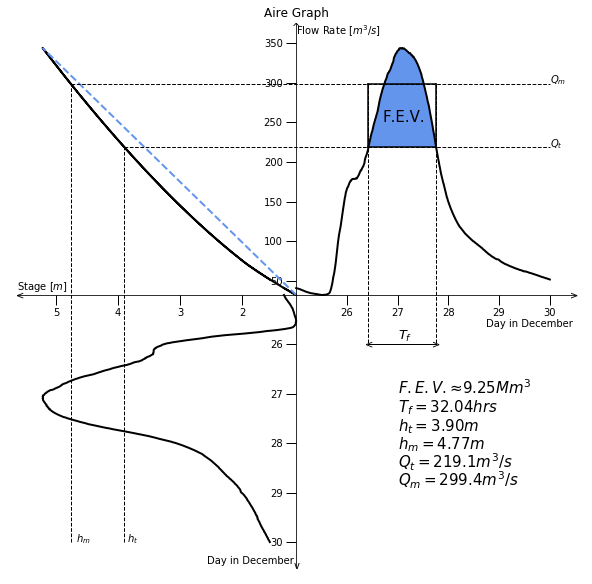
\includegraphics[scale=0.45]{Aire-Quadrant_Graph.png}
\caption{Graph detailing the relationship between the height and flow rate of the River Aire during the 2015 Boxing Day floods using data provided by the Environment Agency from the monitoring station 'Armley'.}
\end{center}
\end{figure}
\begin{table}[H]
\centering
\begin{tabular}{|l|l|l|l|l|}
\hline
Lower Stage Limit {[}m{]} & Upper Stage Limit {[}m{]} & c & b & a \\
\hline
0.2 & 0.685 & 30.69 & 1.115 & 0.156 \\
0.685 & 1.917 & 27.884 & 1.462 & 0.028 \\
1.917 & 4.17 & 30.127 & 1.502 & 0.153 \\
\hline
\end{tabular}
\caption{Aire}
\end{table}
\subsubsection{Past and planned mitigation projects in Leeds}

\subsection{The River Calder}
\begin{figure}[H]
\begin{center}
\includegraphics[scale=0.45]{Calder-Long_Time_Graph.png}
\caption{Graph detailing the relationship between the height and flow rate of the River Aire during the 2015 Boxing Day floods using data provided by the Environment Agency from the monitoring station 'Armley'.}
\end{center}
\end{figure}
\begin{figure}[H]
\begin{center}
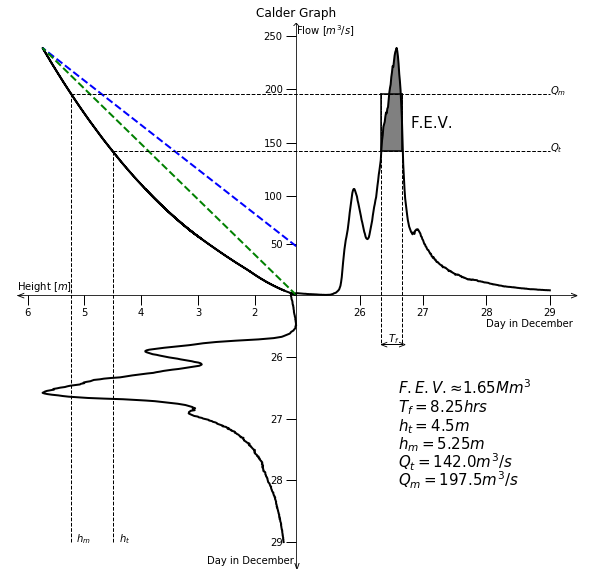
\includegraphics[scale=0.45]{Calder-Quadrant_Graph.png}
\caption{Graph detailing the relationship between the Height and Flow Rate of the River Calder during the 2015 Boxing Day floods using data provided by the Environment Agency from the monitoring station 'Mytholmroyd'.}
\end{center}
\end{figure}
\begin{table}[H]
\centering
\begin{tabular}{|l|l|l|l|l|}
\hline
Lower Stage Limit {[}m{]} & Upper Stage Limit {[}m{]} & c & b & a \\
\hline
0 & 2.107 & 8.459 & 2.239 & 0.342 \\
2.107 & 3.088 & 21.5 & 1.37 & 0.826 \\
3.088 & 5.8 & 2.086 & 2.515 & -0.856 \\
\hline
\end{tabular}
\caption{Calder}
\end{table}
\subsubsection{Past and planned mitigation projects in Calderdale}


\section{The June 2007 flood of the River Don}
\begin{figure}[H]
\begin{center}
\includegraphics[scale=0.45]{Don-Long_Time_Graph.png}
\caption{Graph detailing the relationship between the height and flow rate of the River Aire during the 2015 Boxing Day floods using data provided by the Environment Agency from the monitoring station 'Armley'.}
\end{center}
\end{figure}
\begin{figure}[H]
\begin{center}
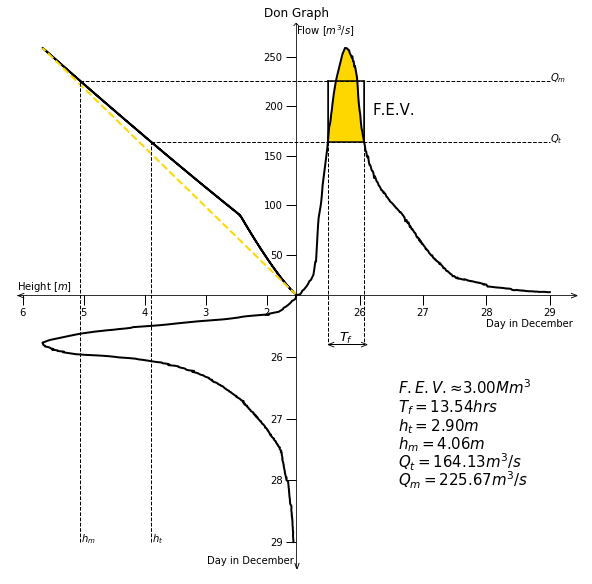
\includegraphics[scale=0.45]{Don-Quadrant_Graph.png}
\caption{Graph detailing the relationship between the Height and Flow Rate of the River Don during the 2015 Boxing Day floods using data provided by the Environment Agency from the monitoring station 'Sheffield Hadfields'.}
\end{center}
\end{figure}
\begin{table}[H]
\centering
\begin{tabular}{|l|l|l|l|l|}
\hline
Lower Stage Limit {[}m{]} & Upper Stage Limit {[}m{]} & c & b & a \\
\hline
0 & 0.52 & 78.4407 & 1.7742 & 0.223 \\
0.52 & 0.931 & 77.2829 & 1.3803 & 0.3077 \\
0.931 & 1.436 & 79.5956 & 1.2967 & 0.34 \\
1.436 & 3.58 & 41.3367 & 1.1066 & -0.5767 \\
\hline
\end{tabular}
\caption{Don}
\end{table}
\subsection{Past and planned mitigation projects in Sheffield}

\section{The November 2012 flood of the River Avon}
\subsection{The flood in Stratford-upon-Avon}
\begin{figure}[H]
\begin{center}
\includegraphics[scale=0.45]{Stratford-Long_Time_Graph.png}
\caption{Graph detailing the relationship between the height and flow rate of the River Aire during the 2015 Boxing Day floods using data provided by the Environment Agency from the monitoring station 'Armley'.}
\end{center}
\end{figure}

\begin{figure}[H]
\centering
\subfloat[Figure 5]{\includegraphics[scale=0.45]{Stratford-Quadrant_Graph_3.png}}
\hfill
\subfloat[Figure 5 plotted using raw flow rate data]{\includegraphics[scale=0.45]{Stratford-Quadrant_Graph_4.png}}
\caption{Comparison of the Warwick graph, the left using our rating information to find our flow rate values and the right using raw flow rate data.}
\end{figure}

\begin{table}[H]
\centering
\begin{tabular}{|l|l|l|l|l|}
\hline
Lower Stage Limit {[}m{]} & Upper Stage Limit {[}m{]} & c & b & a \\
\hline
0.136 & 0.938 & 158.04 & 2.85438 & 0.262919 \\
0.938 & 1.427 & 87.0362 & 0.962129 & 0.358741 \\
\hline
\end{tabular}
\caption{Stratford-upon-Avon}
\end{table}
\begin{figure}[H]
\centering
\subfloat[Figure 5]{\includegraphics[scale=0.45]{Stratford-Square_Lake.png}}
\hfill
\subfloat[Figure 5 plotted using raw flow rate data]{\includegraphics[scale=0.45]{Stratford-FEV_ht_Graph.png}}
\caption{Comparison of the Warwick graph, the left using our rating information to find our flow rate values and the right using raw flow rate data.}
\end{figure}

\subsection{The flood in Warwick}
\begin{figure}[H]
\begin{center}
\includegraphics[scale=0.45]{Warwick-Long_Time_Graph.png}
\caption{Graph detailing the relationship between the height and flow rate of the River Aire during the 2015 Boxing Day floods using data provided by the Environment Agency from the monitoring station 'Armley'.}
\end{center}
\end{figure}

\begin{figure}[H]
\centering
\subfloat[Figure 5]{\includegraphics[scale=0.45]{Warwick-Quadrant_Graph_3.png}}
\hfill
\subfloat[Figure 5 plotted using raw flow rate data]{\includegraphics[scale=0.45]{Warwick-Quadrant_Graph_4.png}}
\caption{Comparison of the Warwick graph, the left using our rating information to find our flow rate values and the right using raw flow rate data.}
\end{figure}

\begin{table}[H]
\centering
\begin{tabular}{|l|l|l|l|l|}
\hline
Lower Stage Limit {[}m{]} & Upper Stage Limit {[}m{]} & c & b & a \\
\hline
0.960 & 3.000 & 40.6178 & 1.44854 & 0.917837 \\
\hline
\end{tabular}
\caption{Warwick}
\end{table}
\begin{figure}[H]
\centering
\subfloat[Figure 5]{\includegraphics[scale=0.45]{Warwick-Square_Lake1.png}}
\hfill
\subfloat[Figure 5 plotted using raw flow rate data]{\includegraphics[scale=0.45]{Warwick-FEV_ht_Graph.png}}
\caption{Comparison of the Warwick graph, the left using our rating information to find our flow rate values and the right using raw flow rate data.}
\end{figure}

\section{Flood-mitigation assessment using FEV}
\subsection{Past and planned mitigation projects upstream of Stratford-upon-Avon}
\subsection{Natural flood management}
\subsubsection{Flow-attenuation features}
\subsubsection{Tree planting}
\subsection{Storage of flood water in reservoirs}
\subsection{Giving room to the River}
\begin{figure}[H]
\centering
\subfloat[Figure 5]{\includegraphics[scale=0.45]{GRR-1.png}}
\hfill
\subfloat[Figure 5 plotted using raw flow rate data]{\includegraphics[scale=0.45]{GRR-2.png}}
\caption{Comparison of the Warwick graph, the left using our rating information to find our flow rate values and the right using raw flow rate data.}
\end{figure}

\section{Precipitation scenarios}

\section{Futher Reading}

\section{Summary and discussion}
\subsection{Acknowledgements}

\section{References}
\begin{thebibliography}{}
\bibitem{1}The Flood and Coastal Defence project of the Forsight programme2004: Foresight, Future Flooding. Archived at https://assets.publishing.service.gov.uk/government/uploads/system/uploads/attachment\textunderscore\\data/file/300332/04-947-flooding-summary.pdf
\bibitem{2}The Telegraph 2015: UK flooding: cost of damage to top £5bn but many homes and businesses underinsured. https://www.telegraph.co.uk/finance/economics/12071604/UK-flooding-cost-of-damage-to-top-5bn-but-many-homes-and-businesses-underinsured.html
\bibitem{3} Peters, H. 1990: Tattooed Faces and Stilt Houses: Who Were the Ancient Yue? Archived at http://sino-platonic.org/complete/spp017\textunderscore yue.pdf
\bibitem{4}Warwickshire County Council 2016: Surface Water Management Plan Methodology Report. Archived at https://apps.warwickshire.gov.uk/api/documents/WCCC-1039-45
\bibitem{5}Warwickshire County Council 2016: Local Flood Risk Management Strategy. Archived at https://apps.warwickshire.gov.uk/api/documents/WCCC-1039-29
\bibitem{6}Stratford. https://www.gaugemap.co.uk/\#!Detail/47
\bibitem{7}Warwick. https://www.gaugemap.co.uk/\#!Detail/45
\end{thebibliography}

\newpage
\appendix
\section{Appendix}

\end{document}